\documentclass{article}
\usepackage{longtable}
\usepackage{graphicx}  % For adding logos/images
\usepackage{tikz}
\usepackage{fancyhdr}  % For header/footer customization
\usepackage{amsmath}   % For math formatting
\usepackage{geometry}  % For page margin adjustments
\geometry{a4paper, margin=1in}

\usepackage{background}  % To include background patterns (optional)


\definecolor{lightgray}{gray}{0.96}
\definecolor{mintgreen}{rgb}{0.88, 1.0, 0.88}  % Define mint green color
\pagecolor{lightgray}  % Set the entire page to mint green

% \backgroundsetup{
%   scale=1,
%   color=black,
%   opacity=0.1,        % Set opacity to make the pattern subtle
%   angle=0,
%   position=current page.center,
%   contents={
%     \begin{tikzpicture}[remember picture, overlay]
%       \foreach \x in {-15,-14,...,15} {
%         \foreach \y in {-20,-18,...,20} {
%           \node at (\x, \y) {
%             \begin{tikzpicture}
%               \draw[fill=lightgray!40] (90:0.2) -- (162:0.2) -- (234:0.2) -- (306:0.2) -- (378:0.2) -- cycle;
%             \end{tikzpicture}
%           };
%         }
%       }
%     \end{tikzpicture}
%   }
% }

\title{\Huge \textbf{Aarkus Intelligence: \\ Vision for Blockchain Data Analytics}}
\author{
  \textbf{Harsh Gupta} \\
  Founder, Aarkus Intelligence \\
  \texttt{harsh@aarkusintelligence.com}
}
\date{\today}

\pagestyle{fancy}
\fancyhf{}
\fancyhead[L]{Aarkus Intelligence Whitepaper}
\fancyhead[R]{\thepage}
\fancyfoot[C]{Draft 1}

% \usetikzlibrary{shapes.geometric, arrows.meta}

% \tikzstyle{block} = [rectangle, rounded corners, minimum width=3cm, minimum height=1cm, text centered, draw=black, fill=blue!20]
% \tikzstyle{arrow} = [thick,-{Stealth[round]}]
% \tikzstyle{circleblock} = [circle, minimum width=1.5cm, text centered, draw=black, fill=green!20]


\begin{document}

\maketitle
\thispagestyle{empty} % To remove page number on the title page

\begin{abstract}
\textit{
The abstract provides an overview of Aarkus Intelligence, focusing on our mission to empower traders with blockchain-based insights and innovative data analysis tools. This document outlines the architecture, utility, and vision behind Aarkus Intelligence, a platform for smarter decision-making in crypto trading.
}
\end{abstract}

\tableofcontents

\newpage
\section{Introduction}
The explosive growth of blockchain technology has introduced an unprecedented influx of data, creating both opportunities and challenges for traders and investors. With the rise of decentralized finance (DeFi), cryptocurrency trading, and non-fungible tokens (NFTs), blockchain has become a cornerstone for digital assets. However, this same expansion has overwhelmed traders with vast, unstructured data, making it difficult to extract actionable insights.

% \begin{tikzpicture}[node distance=2cm]

%   % Main central block (Aarkus Intelligence)
%   \node (aarkus) [circleblock] {Aarkus Intelligence};
  
%   % Key Features (Real-time Data Capture, AI-Powered Insights, Automated Trade Analysis)
%   \node (data) [block, above left of=aarkus, xshift=-1cm, yshift=1cm] {Real-time Data Capture};
%   \node (ai) [block, above right of=aarkus, xshift=1cm, yshift=1cm] {AI-Powered Insights};
%   \node (trade) [block, below of=aarkus, yshift=-1cm] {Automated Trade Analysis};
  
%   % Blockchain, Wallets, and Assets representations
%   \node (blockchain) [block, below left of=trade, xshift=-1cm, yshift=-1cm] {Blockchain Networks};
%   \node (wallets) [block, below of=trade, yshift=-1cm] {Wallets};
%   \node (assets) [block, below right of=trade, xshift=1cm, yshift=-1cm] {Assets};
  
%   % Arrows connecting the central block to the features
%   \draw [arrow] (aarkus) -- (data);
%   \draw [arrow] (aarkus) -- (ai);
%   \draw [arrow] (aarkus) -- (trade);
  
%   % Arrows connecting the features to Blockchain, Wallets, Assets
%   \draw [arrow] (trade) -- (blockchain);
%   \draw [arrow] (trade) -- (wallets);
%   \draw [arrow] (trade) -- (assets);
  
%   \end{tikzpicture}

At its core, Aarkus Intelligence revolutionizes the trading landscape by providing an automated solution that enables traders to visualize, track, and analyze every trade they make across any blockchain without any manual intervention. By seamlessly capturing and processing blockchain trade data, Aarkus delivers real-time performance insights and trend analysis, empowering traders to make data-driven decisions. Whether managing a single wallet or multiple assets across various chains, Aarkus ensures precision in tracking every trade. Powered by AI, the platform transforms raw blockchain data into strategic intelligence, helping traders uncover patterns, predict trends, and optimize their strategies in a fast-paced, ever-evolving market.

By eliminating the need for manual tracking, Aarkus significantly reduces the complexity of analyzing blockchain activity, allowing traders to focus on optimizing their strategies. The platform’s AI-powered insights provide a deeper understanding of wallet behavior, market trends, and asset movements, offering traders a clear edge in an increasingly competitive market.

Additionally, with rising cryptocurrency scams and fraud, Aarkus Intelligence integrates advanced security analytics to detect anomalies and provide actionable insights to protect traders from malicious activities. The result is a comprehensive tool that not only enhances performance but also ensures the safety and integrity of every trade.

\section{Market Overview}
Discuss the importance of data analytics in trading, blockchain trends, and the competitive landscape.

\section{Vision \& Mission}
Describe the long-term vision and mission of Aarkus Intelligence.

\section{The Aarkus Intelligence Platform}
At the core of Aarkus Intelligence lies its unique ability to deliver a comprehensive and detailed representation of every transaction across any blockchain. This capability allows traders not only to visualize their trades in real time but also to have a precise and clear understanding of the transaction flow, significantly enhancing decision-making processes.

\subsection{Transactions: The Core of Trading}
In the blockchain ecosystem, transactions represent the atomic unit of value exchange. A transaction contains crucial information such as sender and recipient addresses, the asset being transferred, and associated transaction fees. Understanding these components is fundamental to accurate trade representation.

\begin{longtable}{|c|c|c|c|c|c|}
\hline
\textbf{Component} & \textbf{Description} & \textbf{Example Value} \\
\hline
Transaction Hash & Unique ID for the transaction & 0x123abc... \\
\hline
Block Number & Block where the transaction was confirmed & 120034 \\
\hline
Sender Address & Wallet initiating the transaction & 0xabc123... \\
\hline
Recipient Address & Wallet receiving the asset & 0xdef456... \\
\hline
Asset & The asset being transferred & ETH \\
\hline
Transaction Value & Amount of asset being transferred & 2 ETH \\
\hline
Gas Fee & Fee paid for processing the transaction & 0.01 ETH \\
\hline
\end{longtable}

\subsection{Trades: An Abstraction Over Transactions}
While transactions represent the building blocks of blockchain activity, trades are abstractions that bundle multiple transactions. For example, buying ETH with USD is one transaction, and using that ETH to purchase LINK is another. A trade combines these steps into a coherent strategy.

\textbf{Example:}
\begin{itemize}
    \item \textbf{Trade 1}: USD $\rightarrow$ ETH (0.25 ETH bought for 500 USD)
    \item \textbf{Trade 2}: ETH $\rightarrow$ LINK (0.1 ETH used to buy LINK)
    \item Remaining 0.15 ETH stays in the open USD/ETH trade.
\end{itemize}

The trades, based on these transactions, can be visualized as follows:

\scriptsize % Reduce the font size further
% Reduce table width with p{<width>} in longtable
\begin{longtable}{|p{1cm}|p{1.2cm}|p{1.2cm}|p{1.2cm}|p{1.2cm}|p{1.5cm}|p{1.5cm}|p{1.2cm}|p{1.2cm}|p{1.5cm}|}
\hline
\textbf{Trade ID} & \textbf{Pair} & \textbf{Entry Asset} & \textbf{Exit Asset} & \textbf{Amount} & \textbf{Price at Entry} & \textbf{Price at Exit} & \textbf{Status} & \textbf{Profit/Loss} & \textbf{Timestamp} \\
\hline
1 & USD/ETH & USD & ETH & 0.15 ETH & \$2000/ETH & N/A & Open & N/A & 2024-10-11 10:30 UTC \\
\hline
1 & USD/ETH & USD & ETH & 0.1 ETH & \$2000/ETH & \$2200/ETH & Closed & \$20 & 2024-10-11 11:00 UTC \\
\hline
2 & ETH/LINK & ETH & LINK & 0.1 ETH & \$2200/ETH & N/A & Open & N/A & 2024-10-11 11:00 UTC \\
\hline
\caption{Trade Tracking}
\end{longtable}
\normalsize % Return to normal font size

\section{Chained Transactions}
Chained transactions represent a series of linked trades that build upon each other. A transaction such as using ETH to buy LINK opens a new trade while partially closing the previous one. This layered system allows traders to see their positions at multiple levels, reflecting both open and closed positions.

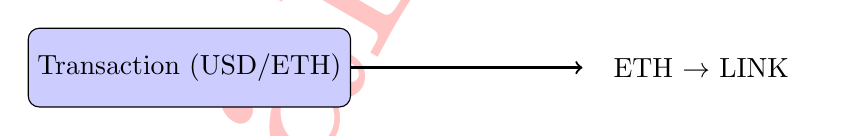
\begin{tikzpicture}[node distance=2.5cm]
  % Main central block (Transaction)
  \node (transaction) [rectangle, rounded corners, minimum width=3cm, minimum height=1cm, text centered, draw=black, fill=blue!20] {Transaction (USD/ETH)};
  
  % Sub blocks for trade flows
  \node (ethlink) [rectangle, rounded corners, minimum width=3cm, minimum height=1cm, right of=transaction, xshift=4cm] {ETH $\rightarrow$ LINK};
  
  % Connecting arrows
  \draw [->, thick] (transaction) -- (ethlink);
\end{tikzpicture}
\subsection{Blockchain Data Analysis}
Explain the core technologies behind real-time wallet tracking, asset performance, and more.

\section{Technology Stack}
\subsection{Analytical Metrics}
Discuss the analytical metrics (e.g., wallet activity, asset performance, trade metrics) and how they assist in making smarter trading decisions.

\section{Tokenomics}
Explain the token model, distribution, and its role in the ecosystem.

\section{Roadmap}
Provide a roadmap for platform development and token launch.

\section{Team}
Introduce the team members and their expertise.

\section{Conclusion}
Summarize the impact of Aarkus Intelligence and the call to action for investors or partners.


\end{document}
